\documentclass[]{article}
\usepackage[T1]{fontenc}
\usepackage[utf8]{inputenc}
\usepackage[english]{babel}

\usepackage{booktabs}
\usepackage{graphicx}

%opening
\title{Travel Salesman Problem: a comparison between exact method, local search and tabu search}
\author{Eduard Bicego}

\includeonly{sections/intro,%
             sections/firstAssignment,%
             sections/secondAssignment,%
             sections/tests,%
             sections/realDomainTests,%
             appendices/instructions
            }

\begin{document}

\maketitle

\begin{abstract}
	In this report is summarized the tests and the results obtained from the development of two programs. These programs solve a Travelling Sales Problem with, respectively, an exact method (using CPLEX library) and Meta Heuristic methods. The programs were a project assignment of the course Methods and Models for Combinatorial Optimization.
\end{abstract}

\section{Introduction}
	The aim of this project is to familiarize with different methods to solve an Asymmetric Travelling Salesman Problem.
	\begin{itemize}
		\item Exact method that gives the optimal solution. This is implemented with the CPLEX API.
		\item Meta heuristic methods: local search and tabu search.
	\end{itemize}

	\subsection{Problem}
		The combinatorial optimization problem was:
		\begin{quote}
				A company produces boards with holes used to build electric frames.  Boards are positioned over a machines and a drill moves over the board, stops at the desired positions and makes the holes.  Once a board is drilled, a new board is positioned and the process is iterated many times.  Given the position of the holes on the board, the company asks us to determine the hole sequence that minimizes the total drilling time, taking into account that the time needed for making an hole is the same and constant for all the holes.
		\end{quote}
	
		This problem can be modelled as an Asymmetric Travelling Salesman Problem. The salesman is represent by the drill and cities by the holes in the board.
	
	\subsection{Document structure}
		The first part of reports show how the exact method, the local search and the tabu search were been implemented with C++ code. In the second part describes the test done and it shows the results obtained. There are two test sections, one with instances originated from random generator and one with real instances generated from real gerber (the standard format for represent PBCs) files.
\section{First Assignment}

	\subsection{Program}
		In order to resolve the Asymmetric Travelling Salesman Problem with the support of CPLEX API I built three files:
		\begin{itemize}
			\item \verb|main|: the file where all other files are linked and combine in order to solve the problem and use CPLEX API;
			\item \verb|dataReader|: in this file the data is read from a file \verb|.dat| given in input at the start of the program;
			\item \verb|ilpSolver|: this file has the responsibility of initialize the environment of CPLEX API with the \verb|setUp| function, in it all the variables and constraints of the mathematical model are initialize. Instead with the \verb|solve| function the program run the CPLEX method for solving a Mixed Integer Programming Problem.
		\end{itemize}


\section{Second Assignment}

\subsection{Program}
	In order to resolve the Asymmetric Travelling Salesman Problem with meta heuristics, I chose to implement the simple Local Search (LC) and the Tabu Search (TS). This choice was done for two reasons: 
	\begin{itemize}
		\item ;
		\item For test my curiosity about this so simple methods for search a good solution in a ridiculous amount of time.
	\end{itemize}

	From the literature we can see that either LS and mostly TS could be change in every details, starting solution, how to choice the neighbor and so on. For these reason I code the program in a modular way.
	
	For an easier testing I write a class SolverExecutor that groups all Solvers and execute sequentially from the starting solution previously set. With this class is easy to modify the Main.cpp file in order to set the environment of test in a few statements.
	
	The main parts are the Solvers interface implemented by LocalSearchSolver and TabuSearchSolver classes. 
	
	The LocalSearchSolver when creates gives the only option:
	\begin{itemize}
		\item the choice of neighbor: Best improvement and First Improvement.
	\end{itemize}
	
	TabuSearchSolver when creates gives the following options:
	\begin{itemize}
		\item The size of tabu list;
		\item The max number of iteration of the algorithm;
		\item The max seconds of execution;
		\item The choice of neighbor: Best Improvement or First Improvement;
		\item The possibility to enable the Aspiration Criteria, a neighbor in the tabu list is chosen if it has a better value of current best solution.
	\end{itemize}

	\subsubsection{When a move is a Tabu}
		After some test I saw that the 

	
\subsection{Calibration}
	For calibration of the Tabu Search algorithm I look only to the tabu list length parameter. Hence I evaluate the test by the result obtained in \textbf{20 seconds} (CPU time). In fact if we increase the size of tabu list we need more time for check if one Move is a tabu.
	
	The test ran with 8 different random start solution, the table\ref{tab:TS-calibration} show the results.
	
	
	\begin{table}
		\centering
		\begin{tabular} {l l l l}
			\toprule
			method & tenure & Obj.Value (avg) & CPU time \\
			\midrule
			Tabu Search & & & \\
			 			& & & \\
			 			& & & \\
			\midrule
			TS Aspiration Criteria & & & \\
		\end{tabular}
		\caption{\label{tab:TS-calibration}Risultati calibrazione Tabu Search}
	\end{table}
	
	



	
\section{Tests and Results}

\subsection{Results Exact Method}

\subsection{Results Local Search}

\subsection{Results Tabu Search}

\subsection{Comparisons of results}
\section{Real Domain tests}
\label{sec:realDomainTests}
	In order to have a better idea of the quality of the methods previously shown I tested them with real instance. These instances are taken from the gerber files avaible from the following online archive:
	\begin{itemize}
		\item \href{https://www.maximintegrated.com/en/design/tools/cad-layout/gerber/}{https://www.maximintegrated.com/en/design/tools/cad-layout/gerber/};
		\item \href{https://www.microchip.com/doclisting/TechDoc.aspx?type=Gerber}{https://www.microchip.com/doclisting/TechDoc.aspx?type=Gerber};
	\end{itemize}

	I explored a dozens of project and select some drill gerber files, from these I made\footnote{This could be done thank to the parser developed by my colleagues Sebastiano Valle and Mirko Bez.} the following \verb|.dat|:
	
	\begin{itemize}
		\item \verb|SC_545|
		\item \verb|MAX_682|
		\item \verb|DS_1120|
	\end{itemize}
	Figure~\ref{fig:SC_545} shows a representation of one of them. The other could be seen from the pdf inside the \verb|RealInstances| folder attached to this report.

	\begin{figure} [h]
		\centering
		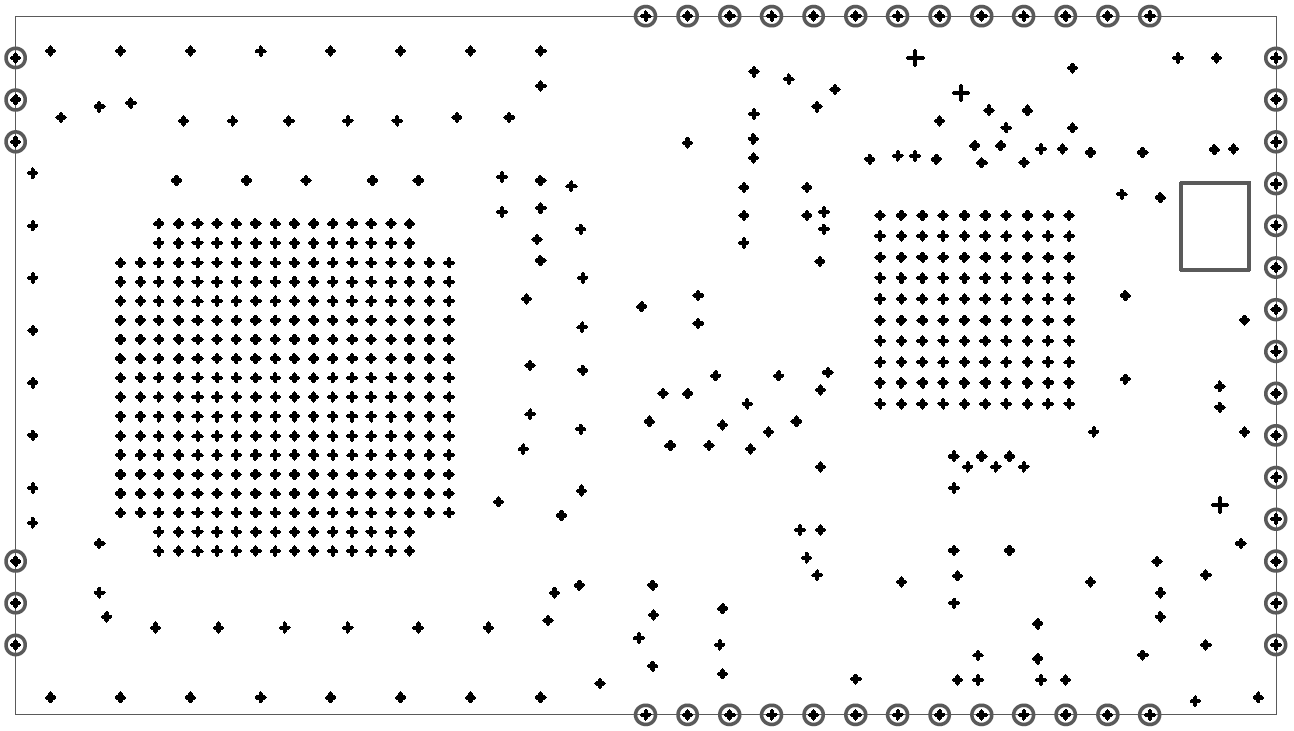
\includegraphics[width=\textwidth]{img/SC_545}
		\caption{The representation of the SC\_545 real instance.}
		\label{fig:SC_545}
	\end{figure}
	
	
	
	\subsection{Results exact method}
		The instances are too huge and the power of computation is too low in order to test the exact method implemented with CPLEX in an amount of time for this project purpose. Neither with a time-out the CPLEX API can give me a intermediate solution in a reasonable amount of time.
		
	\newpage
	
	\subsection{Results Local Search}
		I run the local search with the \textbf{strategy} explained in the previous section \ref{subsec:results-ls}.
		
		
	
	
	\newpage
	
	\subsection{Results Tabu Search}
	
		\subsubsection{Calibration}
			With these new instance the previous calibration is no longer valid. I start from that configuration and I increase the Tabu length.
			
			I made the calibration on \verb|SC_545| instance.
			First I take 8 random initial solution. Then I initialize 4 type of Tabu Search:
			\begin{itemize}
				\item Best Improvement;
				\item Best Improvement with Aspiration Criteria;
				\item First Improvement;
				\item First Improvement with Aspiration Criteria.
			\end{itemize}
			For each type of tabu search I set five different tabu length: 100, 180, 240, 300 and 480. Finally I run each Tabu Search with a maximum time of 30 seconds.  Overall I have $4 \cdot 5 \cdot 8 = 160 $ executions. 
			
			The results are shown in the figure \ref{fig:ri-calibration-sc} and \ref{fig:ri-calibration-sc-avg}.
			
			\begin{figure} [hb]
				\centering
				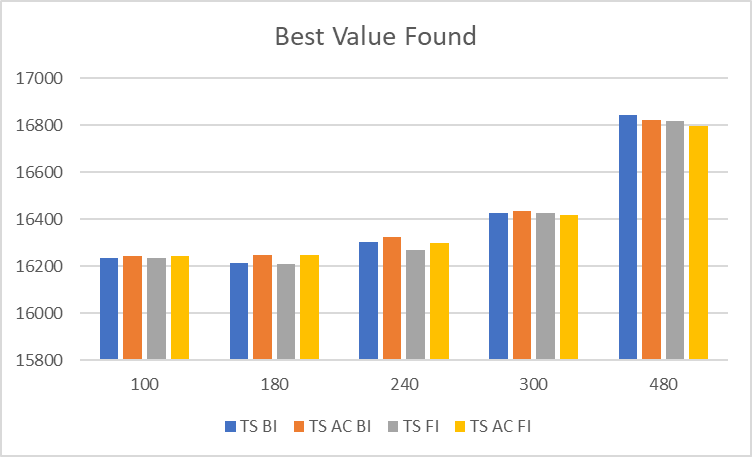
\includegraphics[width=\linewidth]{img/RI-calibration-SC}
				\caption{Calibration Real Instances - best value found.}
				\label{fig:ri-calibration-sc}
			\end{figure}

\newpage	
	
		\begin{figure}[ht]
			\centering
			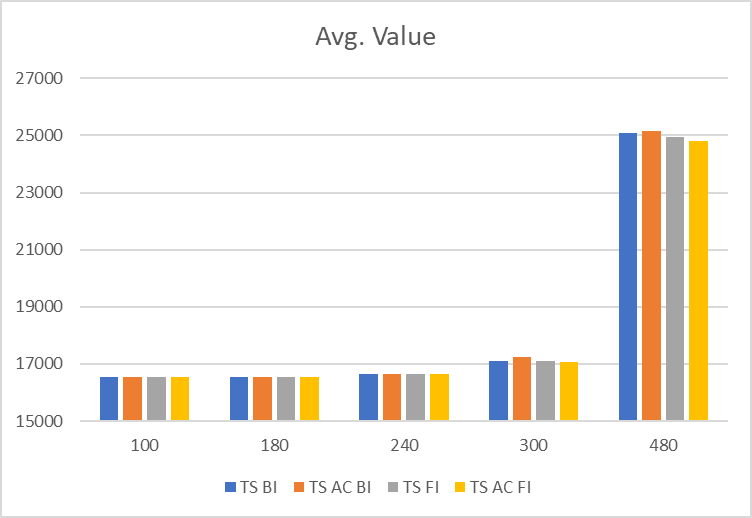
\includegraphics[width=\linewidth]{img/RI-calibration-SC-avg}
			\caption{Calibration Real Instances - Average value}
			\label{fig:ri-calibration-sc-avg}
		\end{figure}
		
			From the charts we can observe that there is some particular differences between the types of Tabu Search. 
			Furthermore we can observe that increasing the tabu length decrease the best value found and also the average of value found. This is suspected, in fact, with tabu length equal to 480, we obtain these because with a tabu list too long the program have a performance bottleneck in the check if a move is a tabu. Hence I start another calibration, only for TS BI AC (choose arbitrarily) with a tabu length equal to 480 and with a maximum time of 300 seconds (5 minutes).
			
			The figure \ref{fig:ri-calibration-tabulengthintime} show with evidence that with more time a larger tabu length is better. If we run a tabu search with tabu length equal to 180 and with a maximum time of 300 seconds we obtain a little improvement but not as the improvement for 480 tabu length case.
			
			\paragraph*{Optimize the code} In order to improve the check if a move is a tabu I substitute the tabu list with two data structures. First I use a \verb|std::list| in order to keep the order of moves inserted into the tabu list. With this data structure I can remove the first element and push back at constant time.
			Second I use a \verb|std::set| for check if a move is a tabu in constant time. I use the concatenation of integer \verb|from| and \verb|to| as key.
			
			\textbf{N.B.} This optimization could brings better result in all the previously test. For limit of time I use the optimization only from now on.
			
			\paragraph*{} With the implementation I execute again some test with TS BI AC with tabu length 180 and 480. The result is that now with 30 seconds I can achieve a better result with tabu length of 480, also the tabu length of 180 have a better solution. In figure ~\ref{fig:ri-calibration-optimize} are shown the comparison between before and after optimization. 
			
			
\newpage		
	
			\begin{figure}
				\centering
				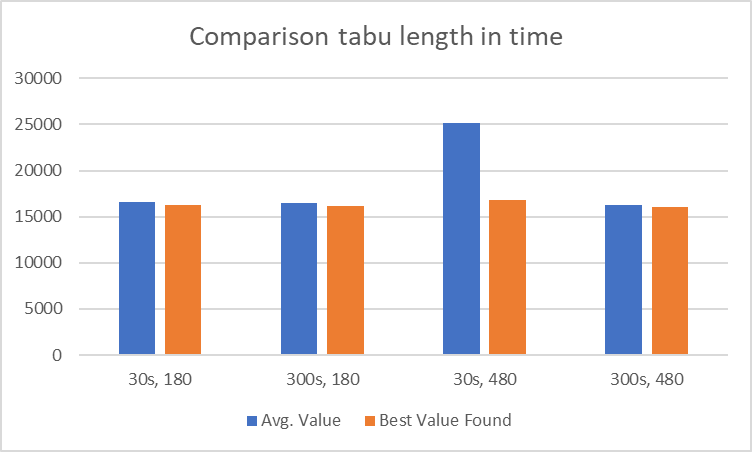
\includegraphics[width=\linewidth]{img/RI-calibration-TabuLengthInTime}
				\caption{Comparison results of TS BI AC with different tabu length and max time.}
				\label{fig:ri-calibration-tabulengthintime}
			\end{figure}
		
			\begin{figure}
				\centering
				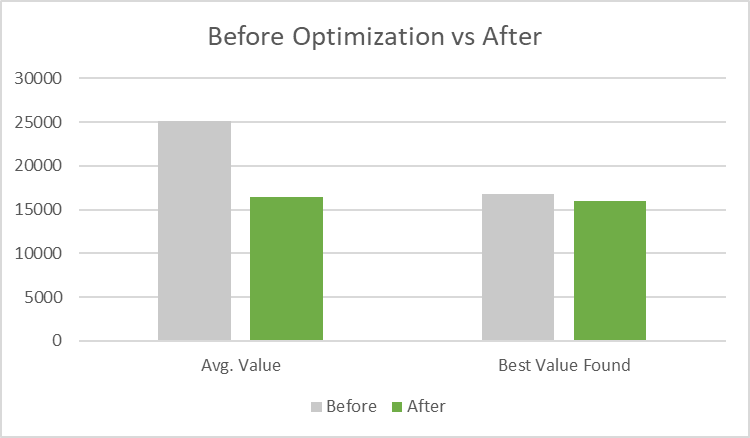
\includegraphics[width=\linewidth]{img/RI-calibration-optimize}
				\caption{Result of TS BI AC in 30 seconds, length of 480, without and with optimization of tabu list.}
				\label{fig:ri-calibration-optimize}
			\end{figure}
		
		
			
			
		
			
			
		
			
		
			
			
			
	
	
	
		
		
	
\appendix
\section{Instructions for run programs}




\end{document}
